\documentclass[11pt]{article}

\newcommand{\cnum}{CS188}
\newcommand{\ced}{Winter 2017}
\newcommand{\ctitle}[3]{\title{\vspace{-0.5in}\cnum, \ced\\Problem Set #1: #2\\Due #3}}
\usepackage{enumitem}
\usepackage{graphicx}
\newcommand{\solution}[1]{{{\color{blue}{\bf Solution:} {#1}}}}
\usepackage[usenames,dvipsnames,svgnames,table,hyperref]{xcolor}

\renewcommand*{\theenumi}{\alph{enumi}}
\renewcommand*\labelenumi{(\theenumi)}
\renewcommand*{\theenumii}{\roman{enumii}}
\renewcommand*\labelenumii{\theenumii.}


\begin{document}
\ctitle{4}{Clustering & PCA}{March 16,2017}
\author{Rohan Varma}
\date{}
\maketitle
\vspace{-0.75in}

\section{Problem 1}
\begin{enumerate}
\item Problem 1a

\solution{
Plot of mean face: \newline{}
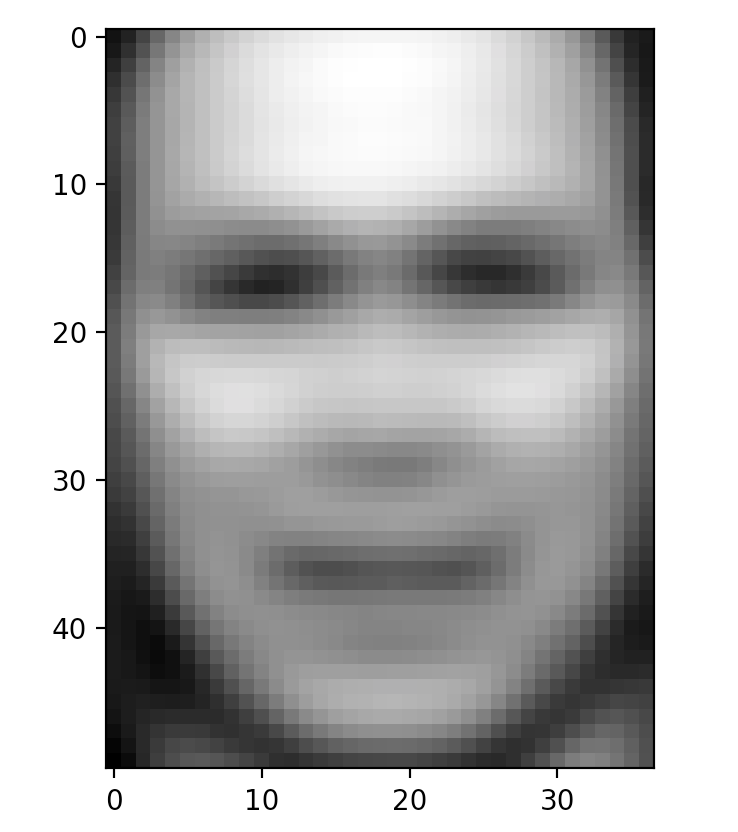
\includegraphics[scale=0.75]{mean_face.png}
\newline{}
This "average" face is much blurrier and much less defined than actual faces in the dataset. Since all pictures in the dataset were human faces, the "average" face retains the general outline of a face, and we can see general outlines of facial features such as the nose, mouth, and eyes. This average face has very poorly defined features (mostly just outlines), which seems to arise from the variation in nose, eye, and mouth structure among all the faces. 
}

\item Problem 1b

\solution{
Top 12 eigenfaces: \newline{}
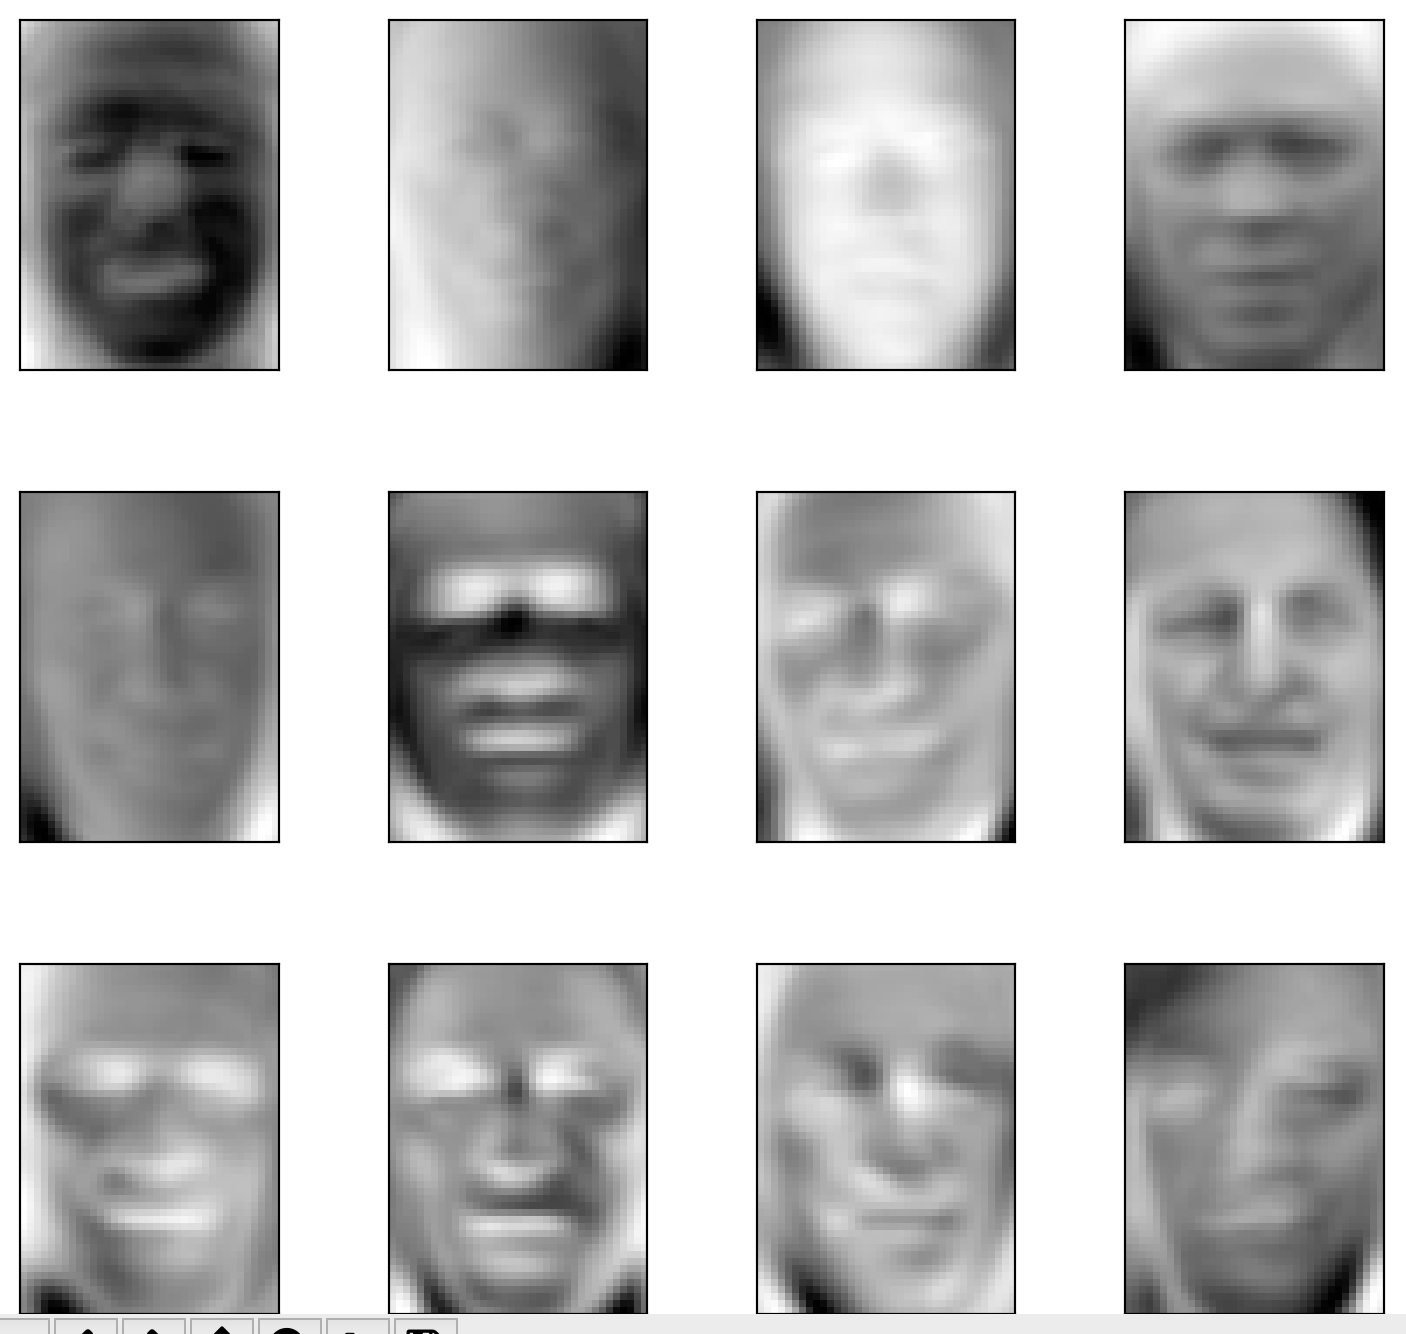
\includegraphics[scale = 0.6]{eigenfaces.png}
\newline{}
The top 12 eigenfaces all vary quite a bit with respect to each other, though their variability seems to decrease for the last few eigenfaces. They represent several different facial features, backgrounds, and lighting graients. The first few eigenfaces are more general while the last few look more defined in comparison. These were chosen as the top 12 eigenfaces since they best represent the entire original training set. A combination of these faces along with the mean face would yield quite good approximations for all faces in the dataset. If we interpret the eigenfaces with respect to variance, then these 12 eigenfaces together capture a significant portion of the variability among faces in the original dataset. These 12 basis vectors capture the top 12 directions of maximal variance. 
}

\item Problem 1c
\solution{
\newline{}
l = 1 gallery \newline{}
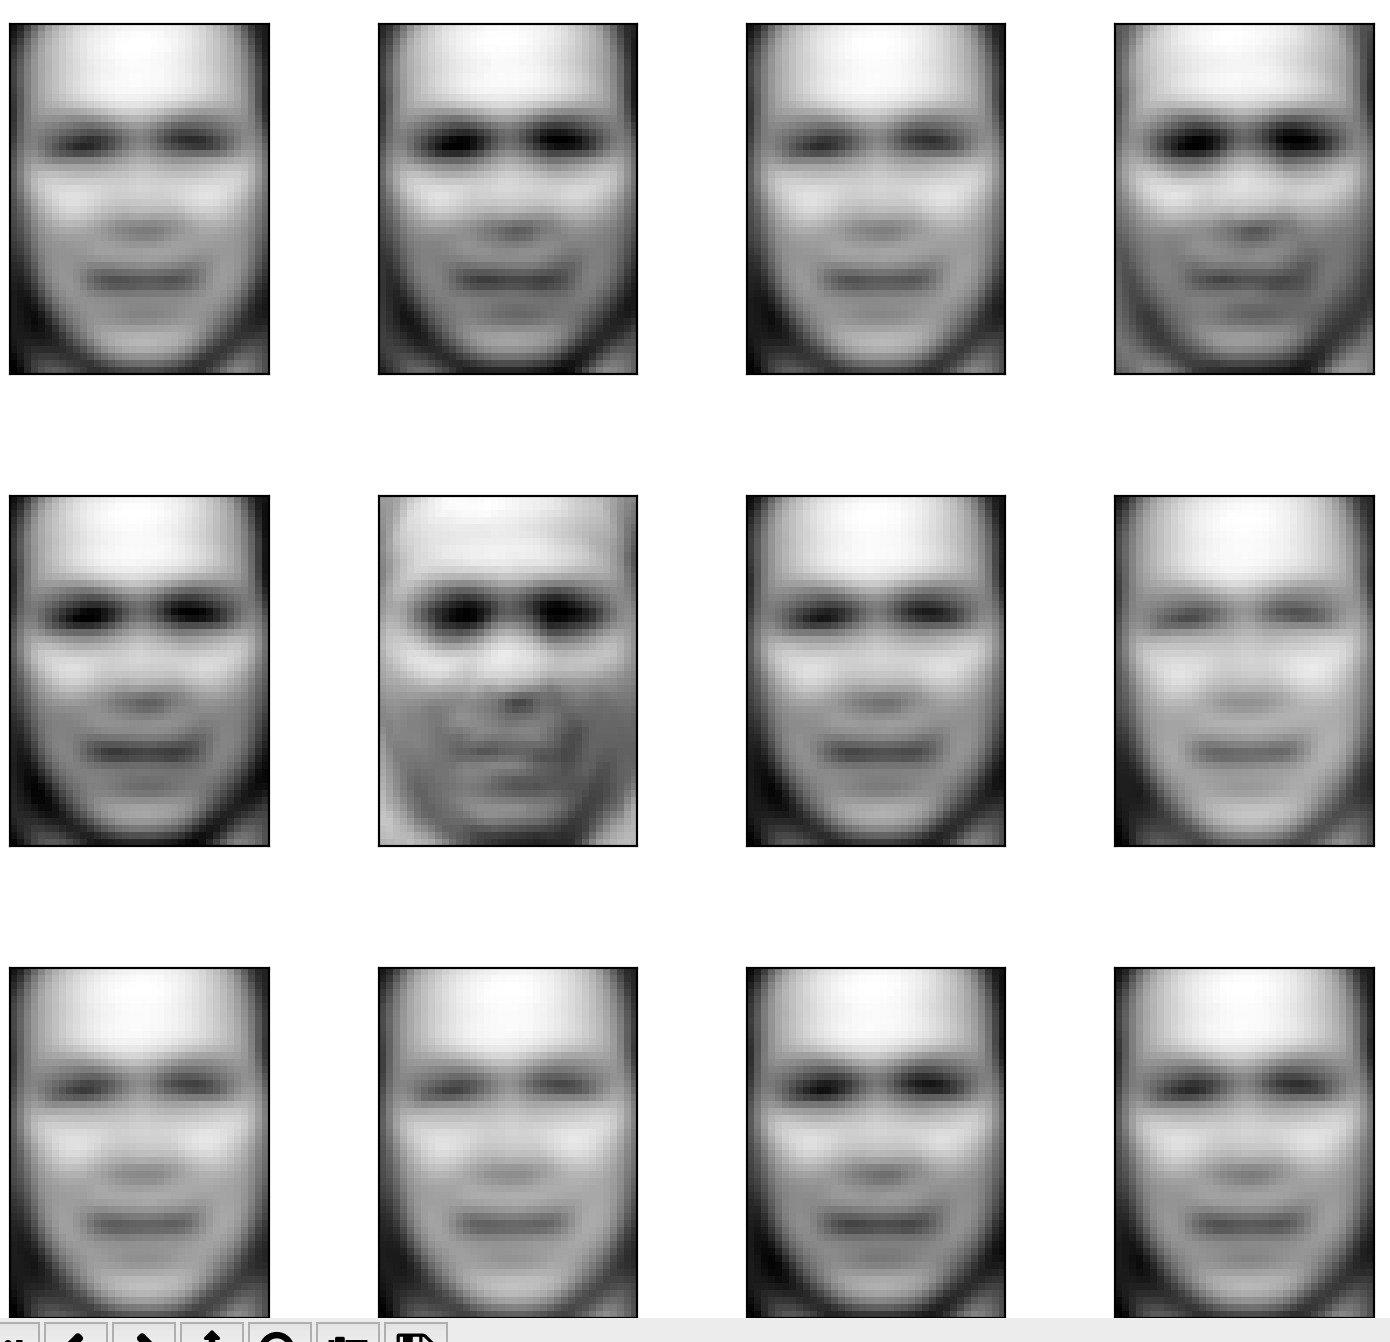
\includegraphics[scale = 0.6]{pca_l=1.png} \newline{} 
\newline{}
l = 10 gallery \newline{}
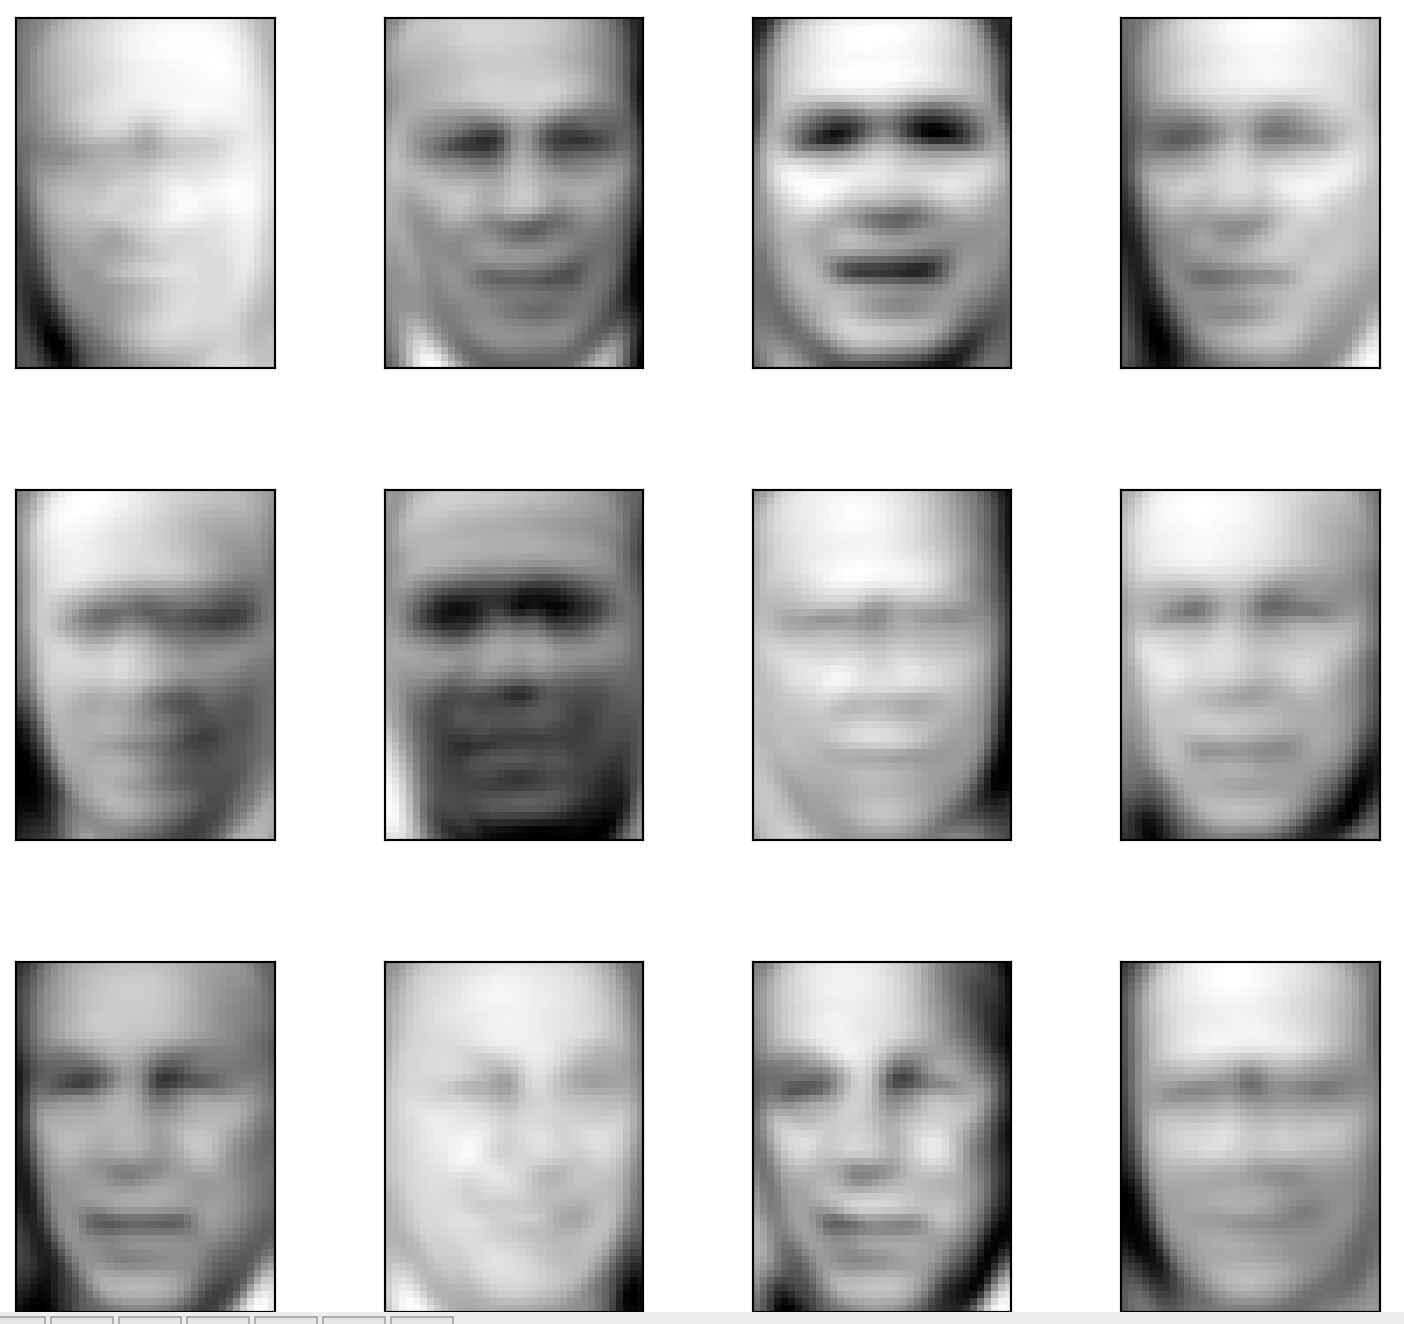
\includegraphics[scale = 0.6]{pca_l=10.png} \newline{} \newpage
l = 50 gallery \newline{}
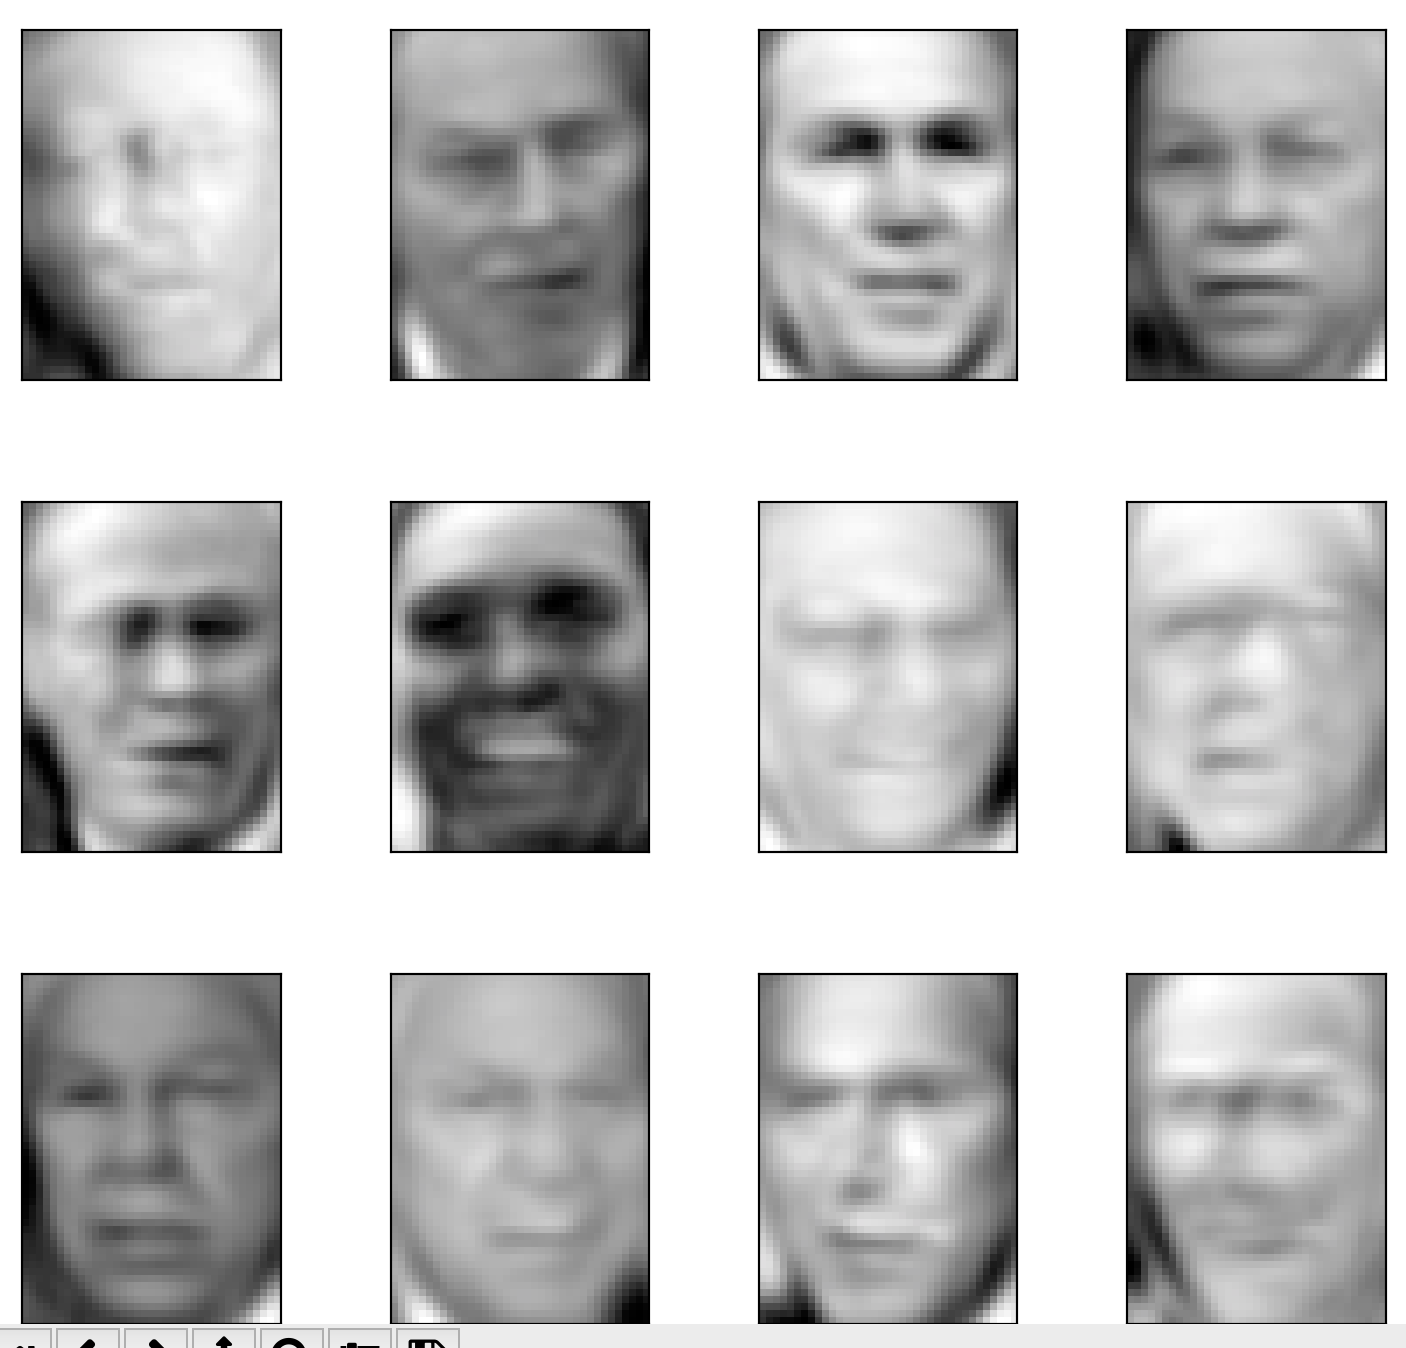
\includegraphics[scale = 0.6]{pca_l=50.png} \newline{} \newpage
l = 100 gallery \newline{}
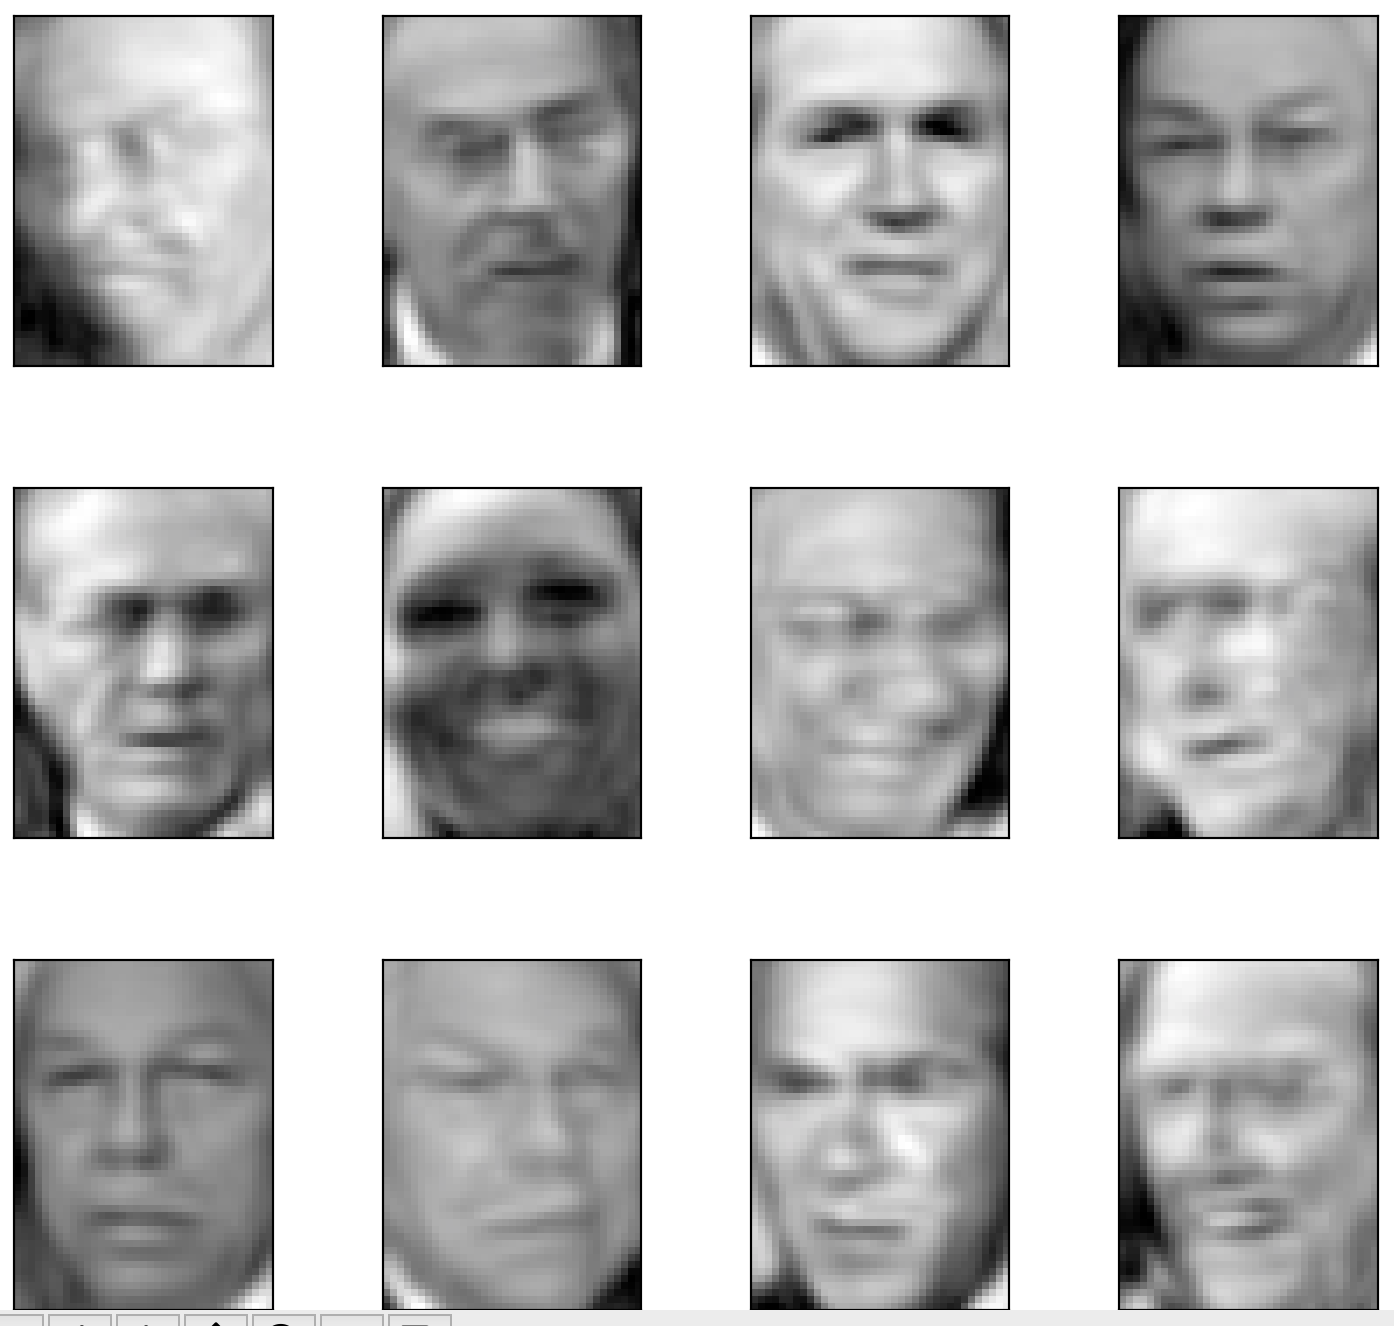
\includegraphics[scale = 0.6]{pca_l=100.png} \newline{} \newpage
l = 500 gallery \newline{}
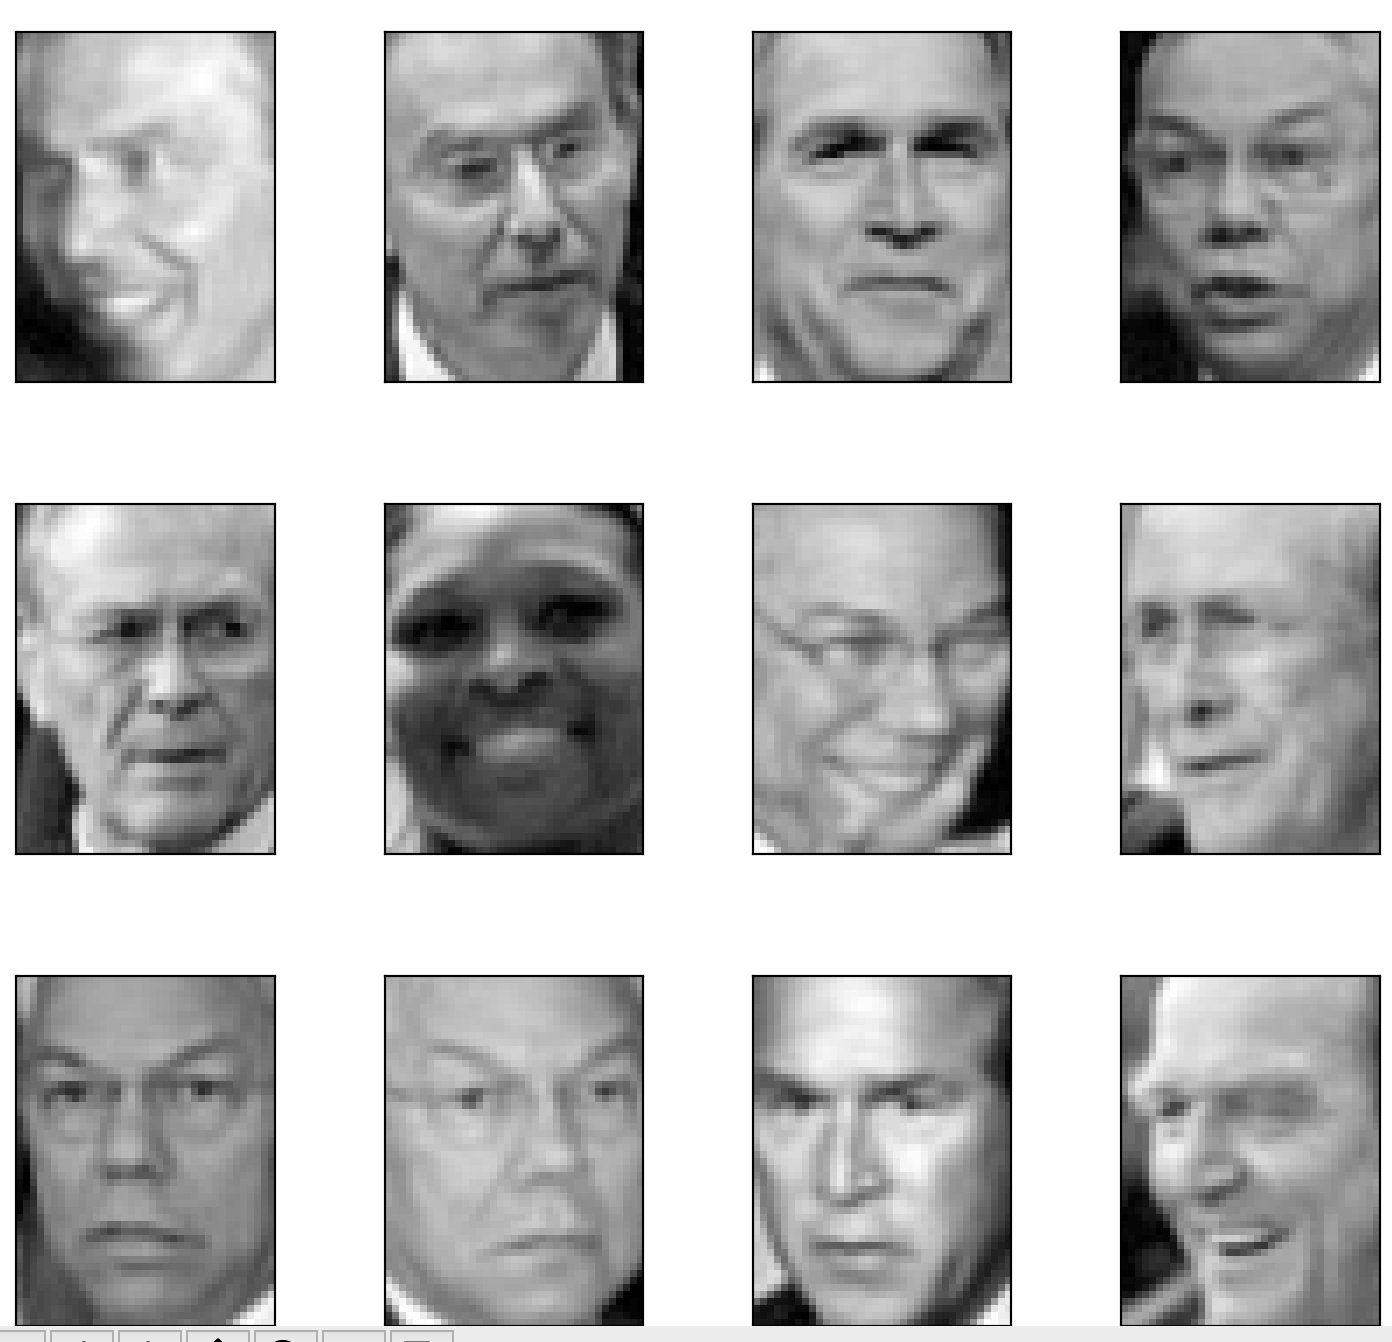
\includegraphics[scale = 0.6]{pca_l=500.png} \newline{} \newpage
l = 1288 gallery \newline{}
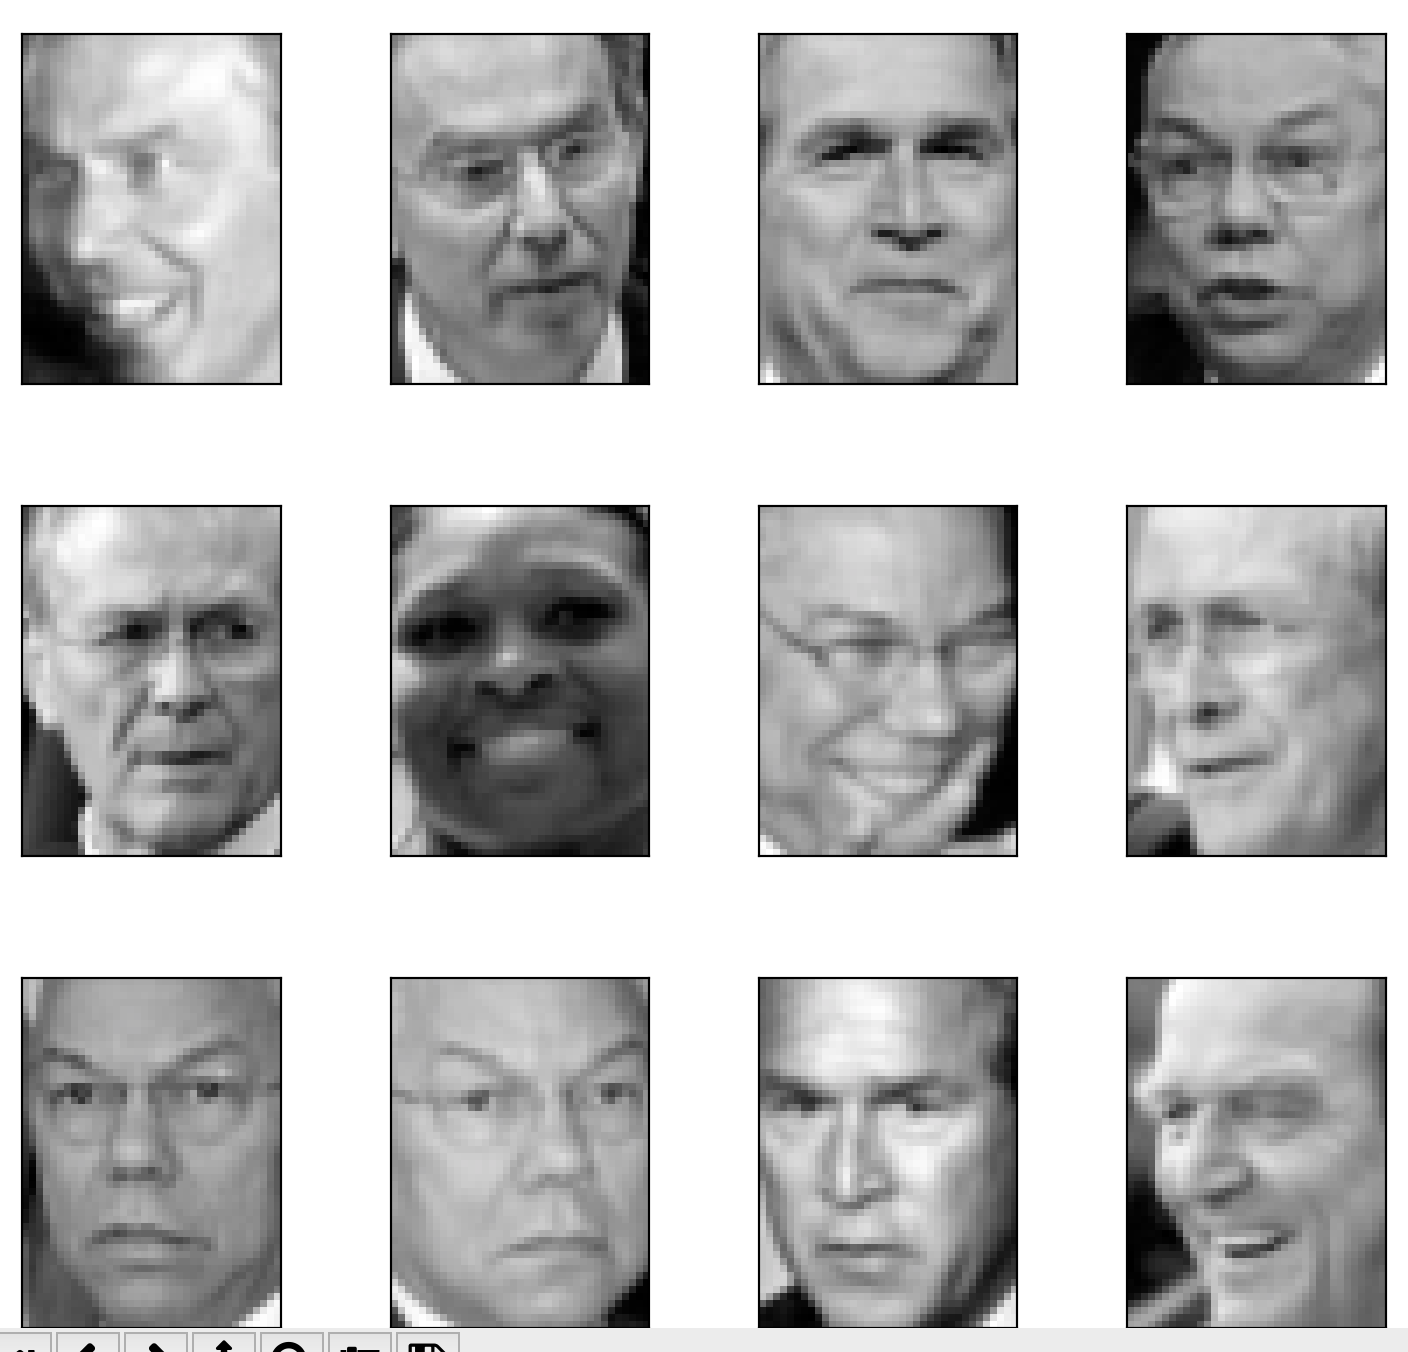
\includegraphics[scale = 0.6]{pca_l=1288.png} \newline{} \newline{}
With smaller values of l, the data is projected onto a very low-dimensional space. For l = 1, for example, the data is represented with only a single feature, so it's essentially impossible to effectively distinguish between faces. For higher values of l, the data is represented with a larger amount of features, so we see increasing variability between the faces, and each face begins to get more and more defined/detailed. With the highest values for l, it is quite easy to distinguish between faces, but this comes at a higher computation cost since we have much more features. Howeover, as l continues to increase, for example from $l = 500$ to $ l = 1288$, the definition/detail of the faces does not increase much, so facial recognition is not easier. However, for the latter, we require almost 800 more principal components, so there's increased dataset size and computation cost with nearly no increase in ease of facial recognition. 
}
\end{enumerate}

\newpage
\section{Problem 2}

\item Problem 2a

\solution{
If we allow $k$, the number of clusters, to be variable, and try to minimize $J(c, \mu, k)$ then we can easily let $k = n$, so we will have n different clusters and each point will be its own cluster. With this, we can get a minimum value of 0. For this to happen, the mean $\mu_j$ for each of the n clusters is just the single point that is assigned to the cluster, so we will have $\mu_j = x_j, j \in {1...n}$. The cluster assignments are $c^{(i)} = i, i \in {1...n}$ since each point is given its own cluster. With these settings, every squared difference can be shown to be 0: \[x^i - \mu_{c^i} = x^i - \mu_i = x^i - x^i = 0\] This is a bad idea since clustering is generally done to understand where similarities occur in our data, and to group data points by how similar they are with respect to each other, and giving each point its own cluster does not accomplish this. 
}
\item Problem 2d

\solution{
Plots for k-means cluster assignments for each iteration using random init: \newline{}
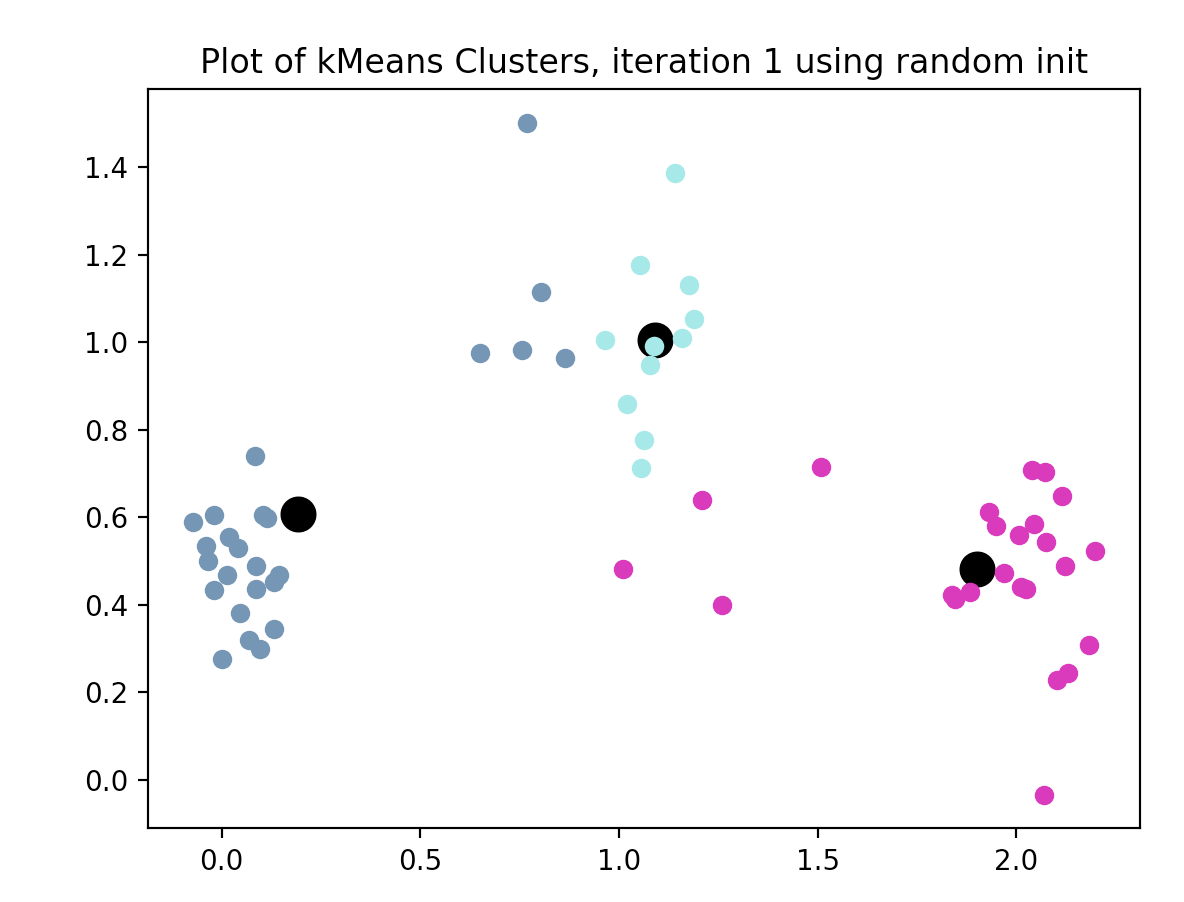
\includegraphics[scale = 0.5]{kmeans-rand-iter-1.png} \newline{}
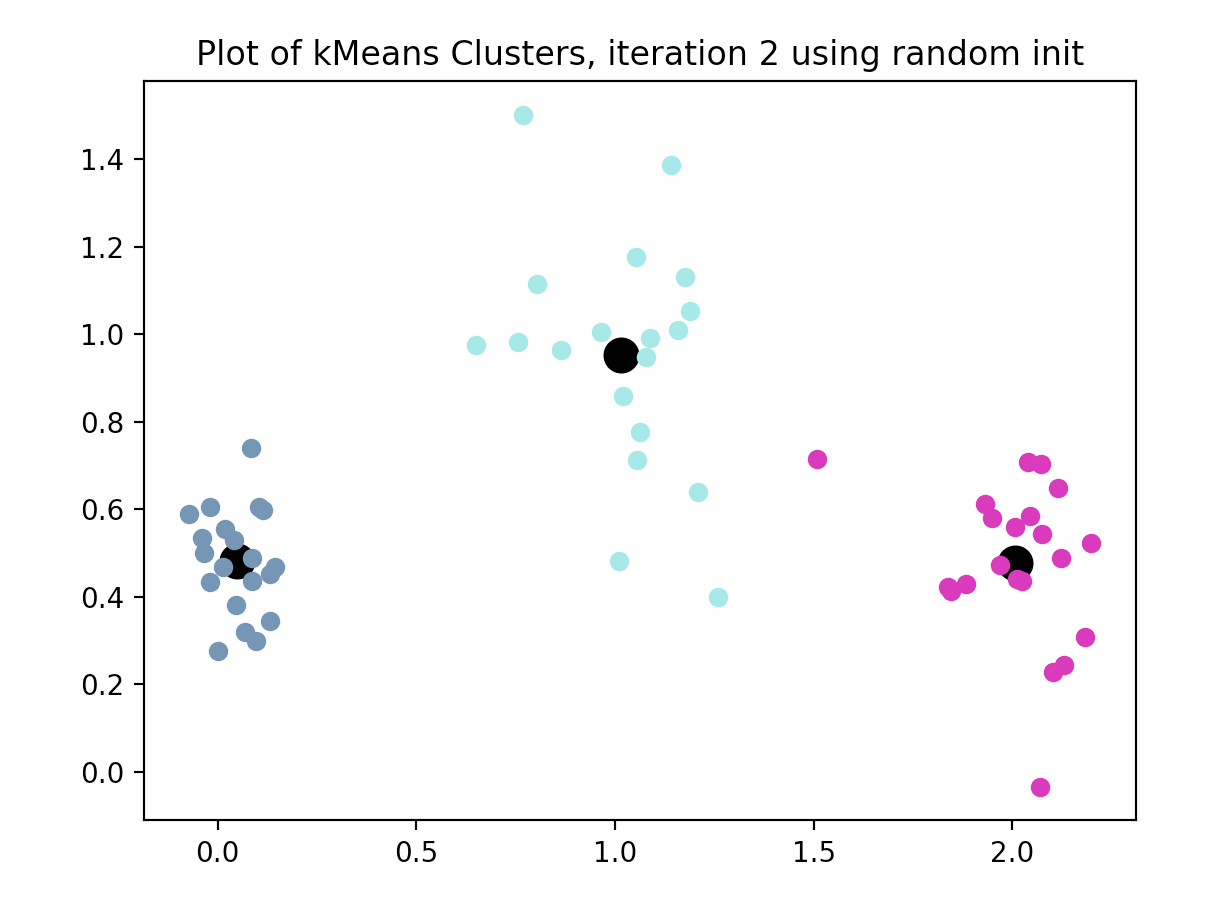
\includegraphics[scale = 0.5]{kmeans-rand-iter-2.png} \newline{}
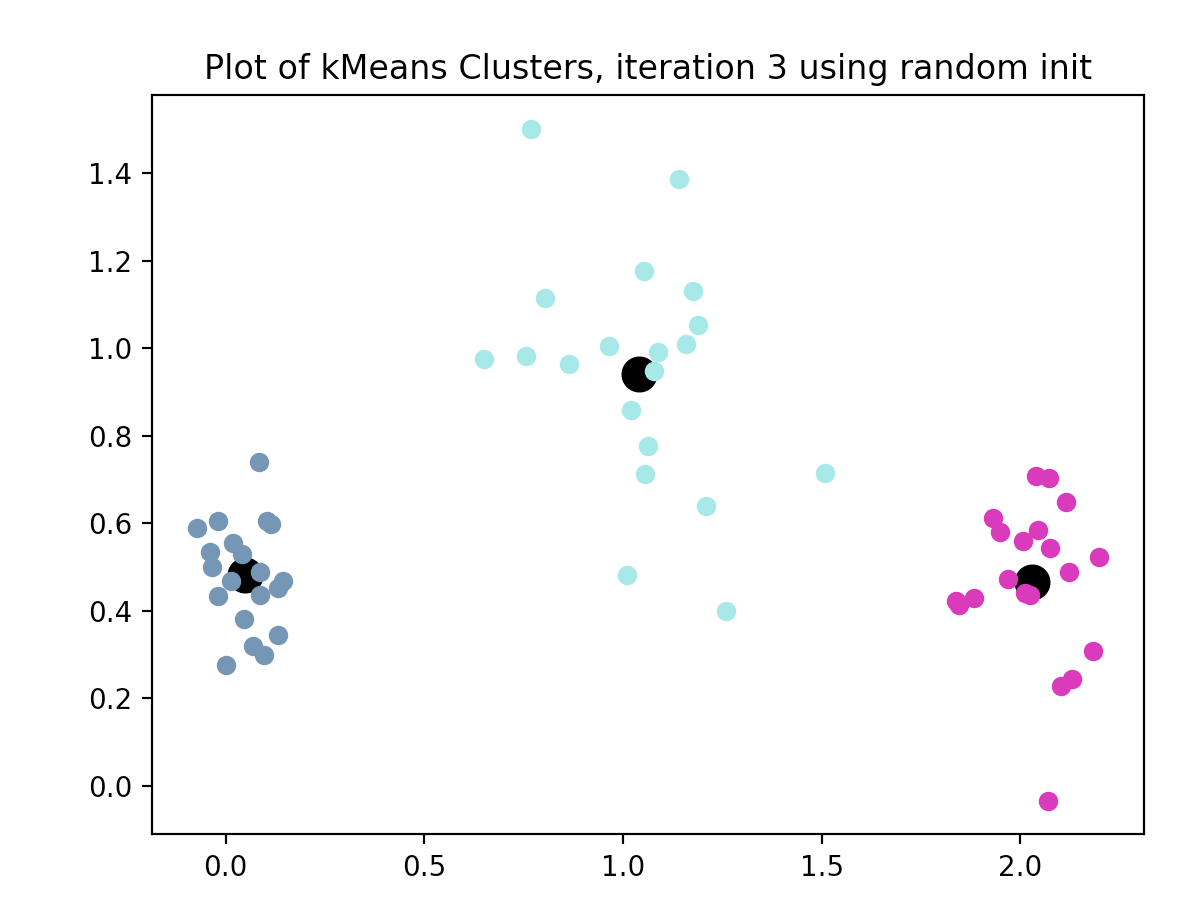
\includegraphics[scale = 0.5]{kmeans-rand-iter-3.png} \newline{}
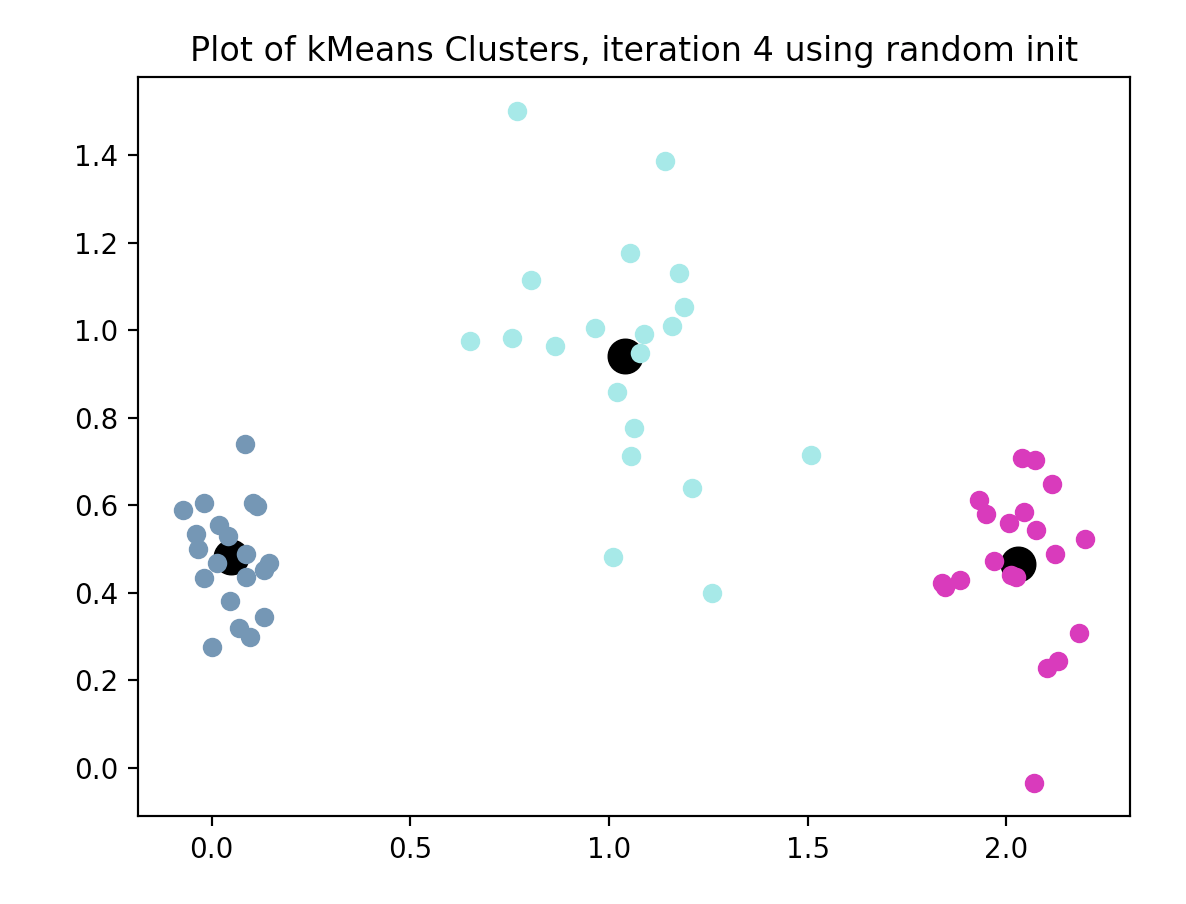
\includegraphics[scale = 0.5]{kmeans-rand-iter-4.png} \newline{}
The algorithm iterates four times, computing clusters based off of previous centroids (in the first iteration, the randomly initialized centroids), and then updating the centroid. The 4th iteration plot is the same as the 3rd iteration plot since the cluster assignments and centroids did not change. My implementation checks if the algorithm should terminate after the call to plot(), hence the plot for the extra iteration. 
}

\item Problem 2e

\solution{
Plots for k-medoids cluster assignments for each iteration using random init: \newline{}
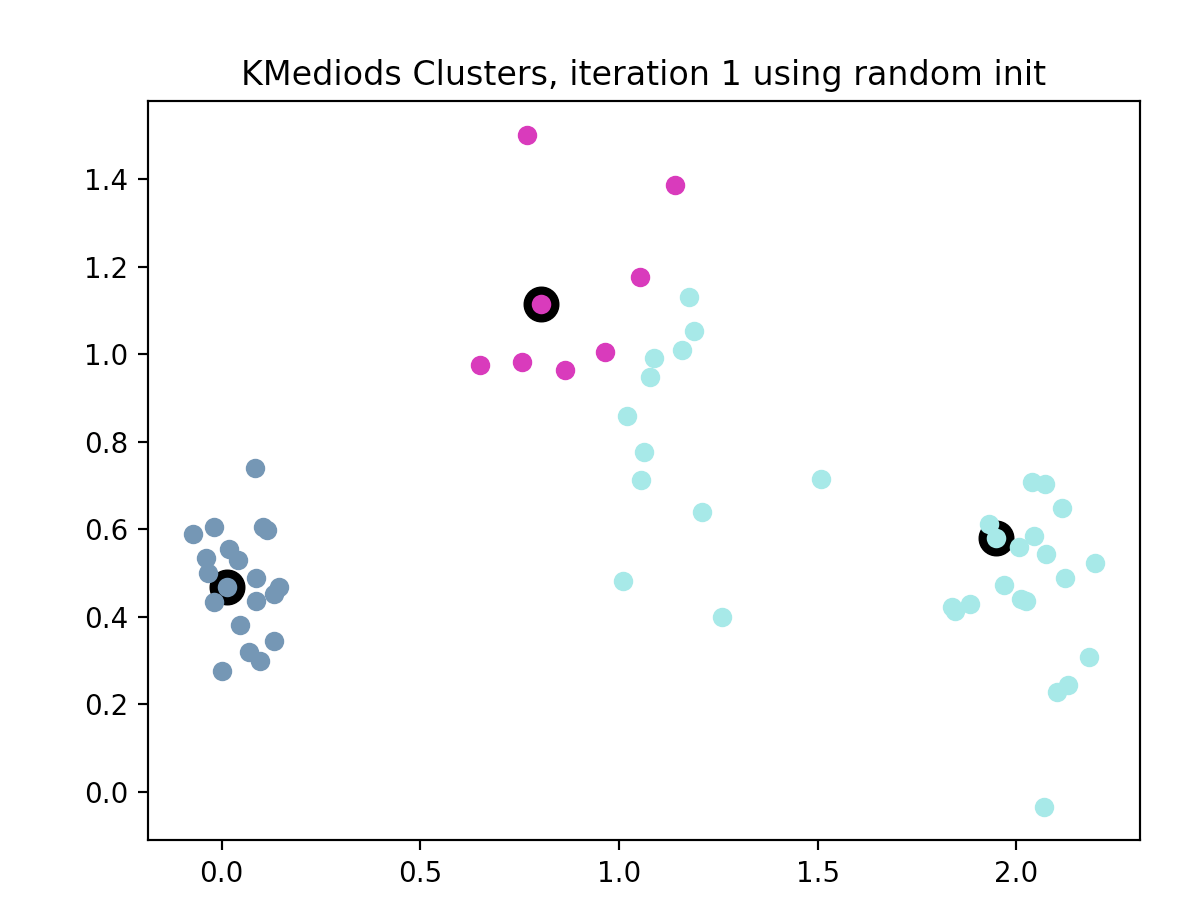
\includegraphics[scale=0.5]{kmed-rand-iter-1.png} \newline{}
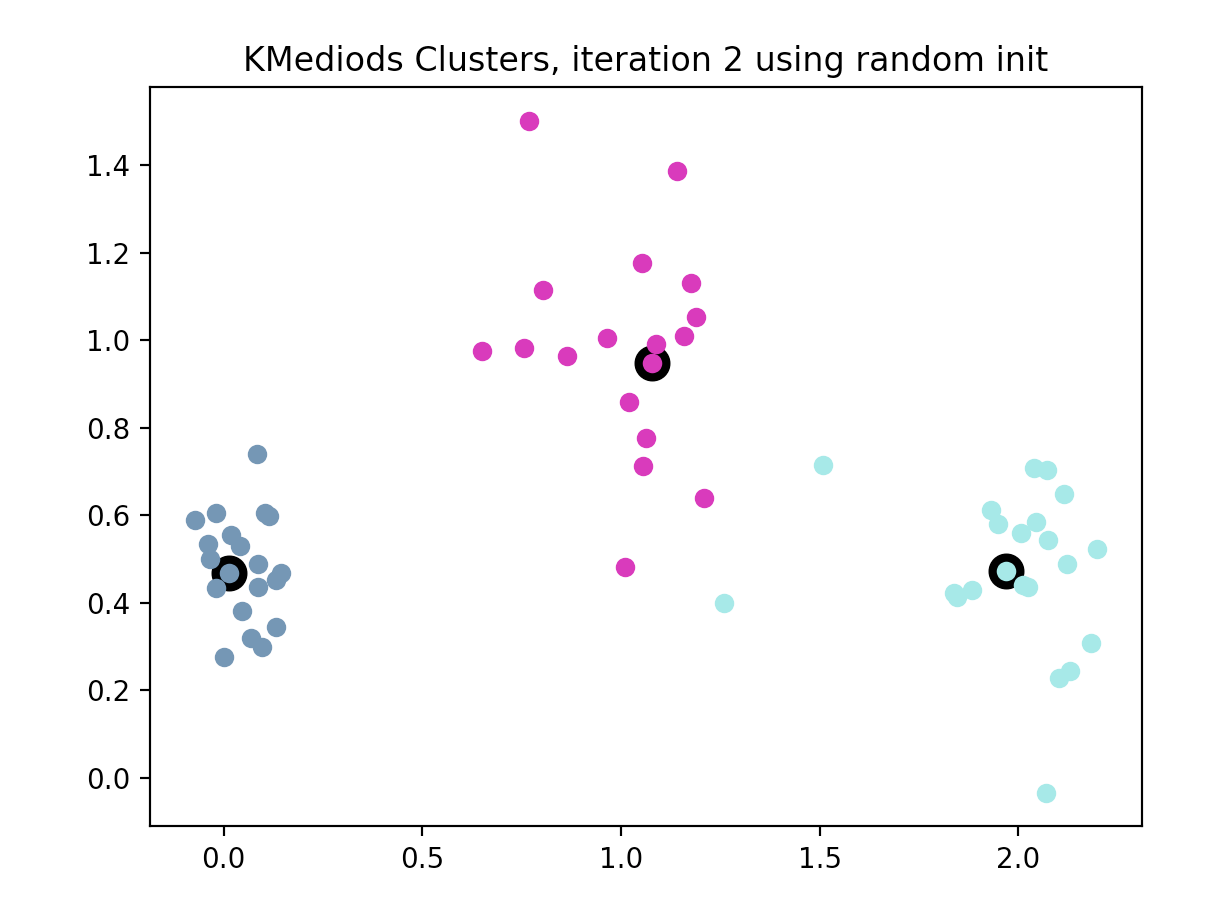
\includegraphics[scale=0.5]{kmed-rand-iter-2.png} \newline{}
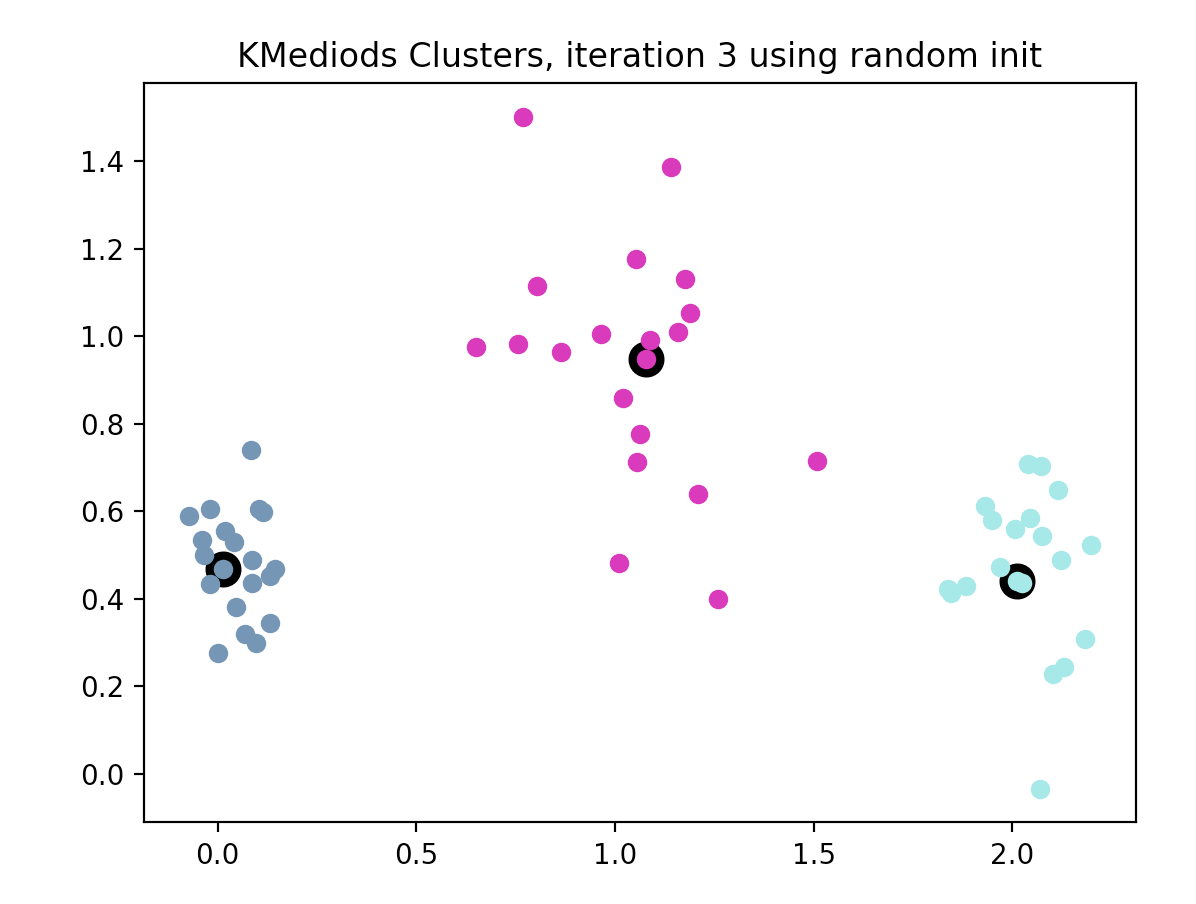
\includegraphics[scale=0.5]{kmed-rand-iter-3.png} \newline{}
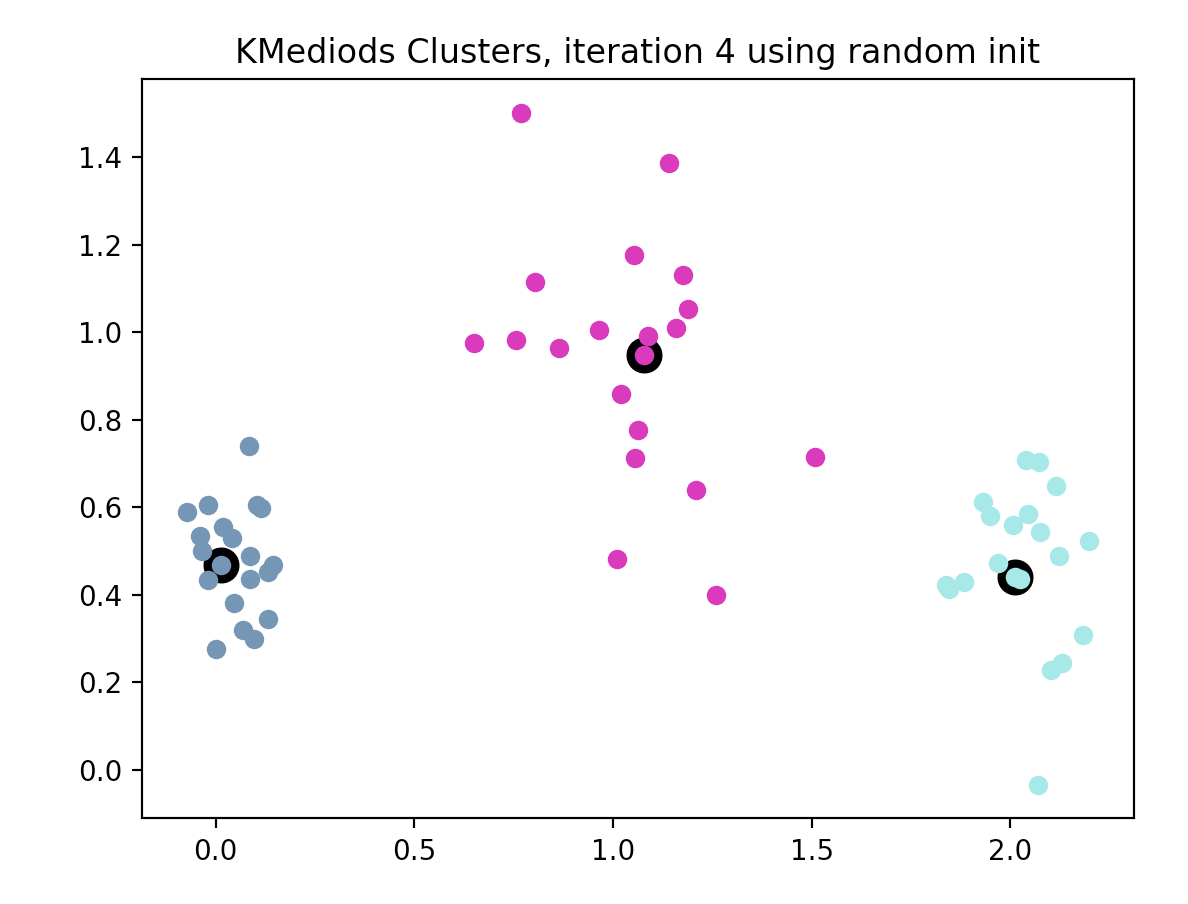
\includegraphics[scale=0.5]{kmed-rand-iter-4.png} \newline{}
The algorithm again iterates four times, computing clusters based off of previous medoids (which is the point whos distance to other points is the least), and then updating the medoids. The 4th iteration plot is once again the same as the 3rd iteration plot since the cluster assignmetns and centroids did not change. My implementation checks if the algorithm should terminate after the call to plot(), hence the plot for the extra iteration. 
}

\item Problem 2f

\solution{
Plots for k means cluster assignments for each iteration using cheat init: \newline{}
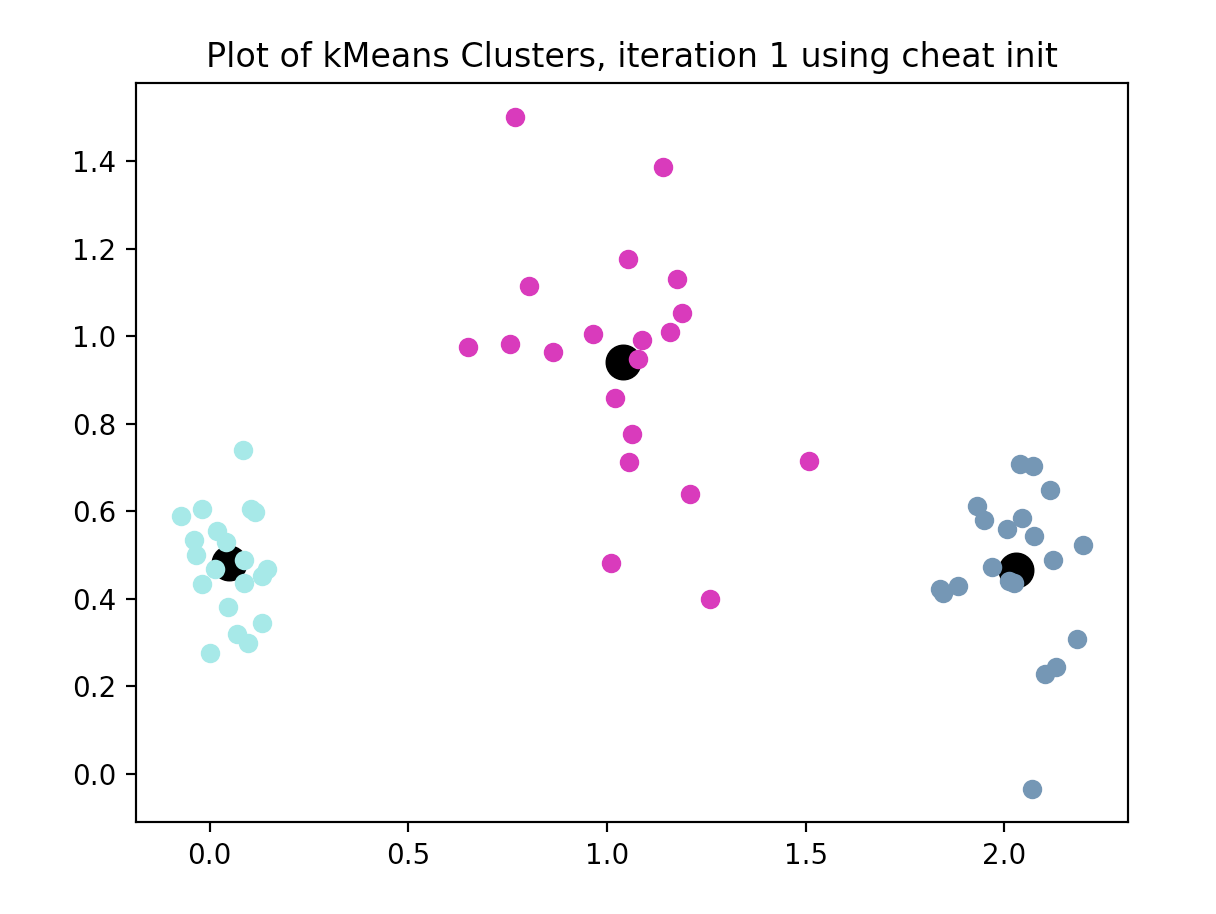
\includegraphics[scale=0.5]{kmeans-cheat-iter-1.png} \newline{}
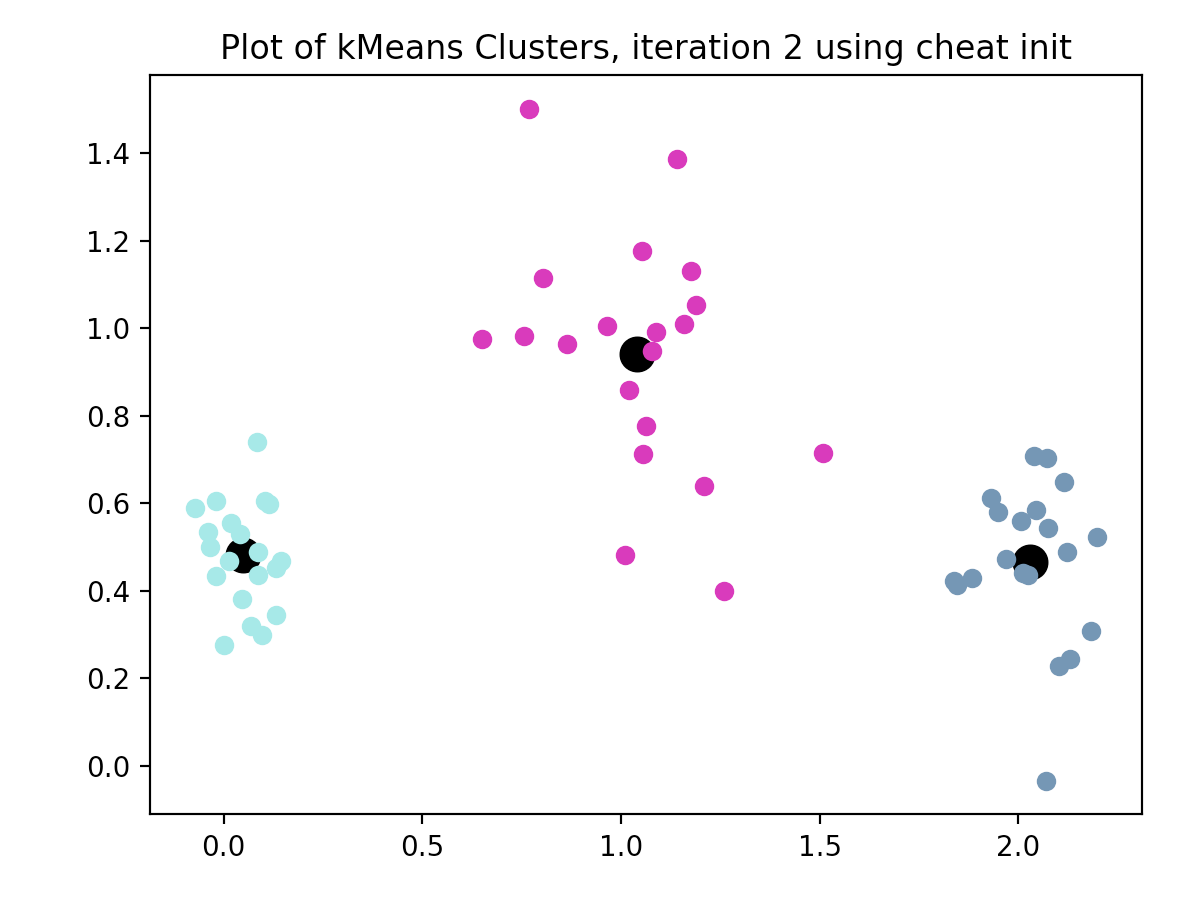
\includegraphics[scale=0.5]{kmeans-cheat-iter-2.png} \newline{}
Plots for k medoids cluster assignments for each iteration using cheat init: \newline{}
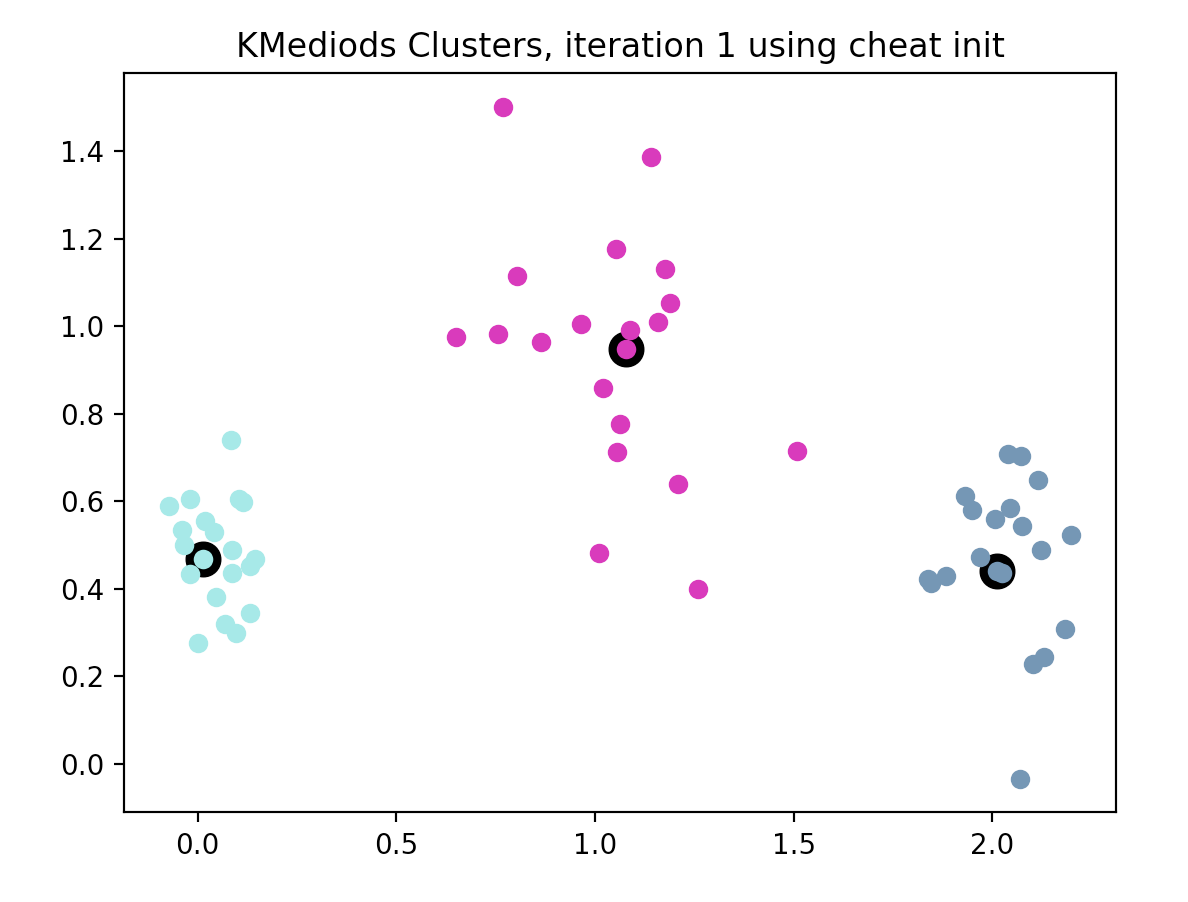
\includegraphics[scale=0.5]{kmed-cheat-iter-1.png} \newline{}
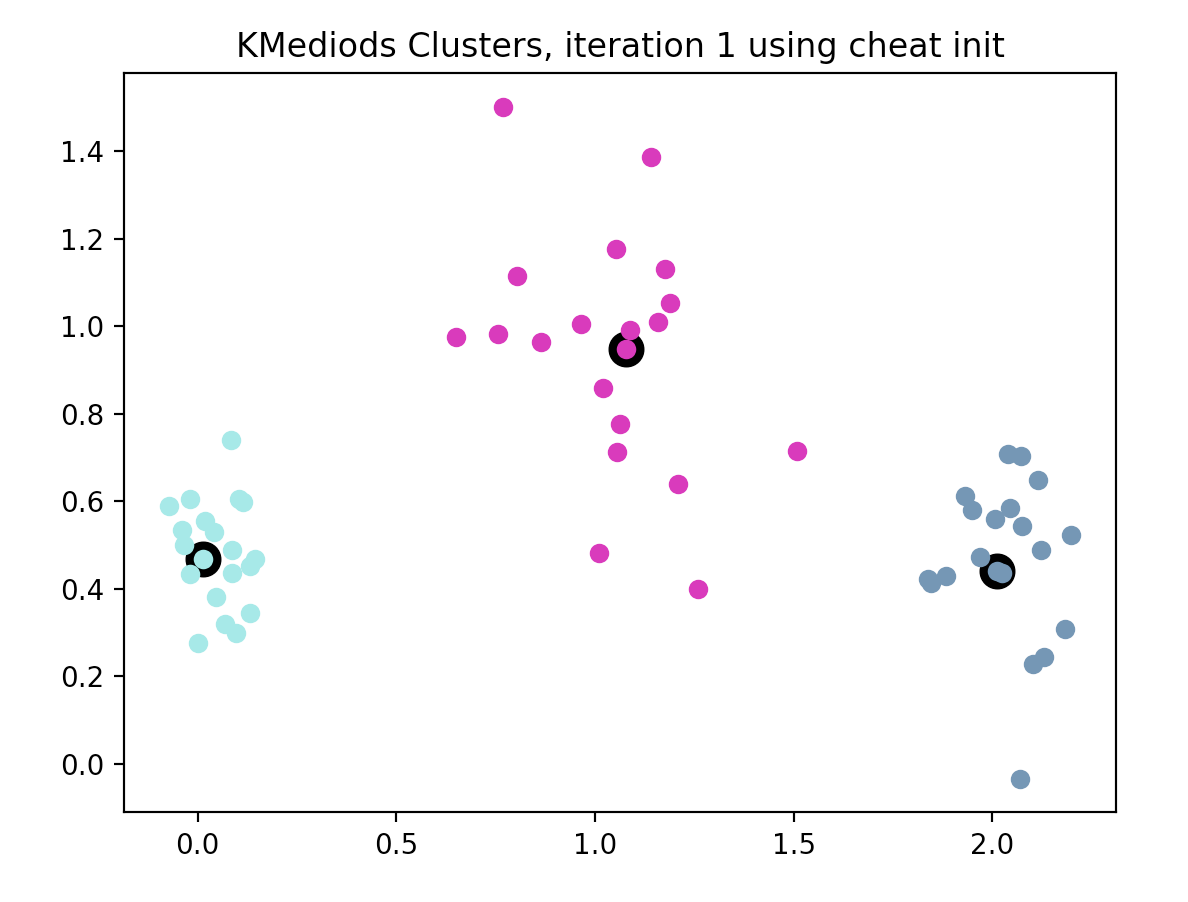
\includegraphics[scale=0.5]{kmed-cheat-iter-1.png} \newline{}
Since cheat init initializes by returning the medoid of clusters that are initially assigned based on the labels, both k means and k medoids clustering converge more quickly than when using random init. In both k-means and k-medoids, the clustering is ideal after the first iteration, and in the second iteration, the assignments and centroids/medoids are not changed, so the algorithm terminates. Once again, for both k-means and k-medoids, the second iteration plot is identical to the first because I call plot() before checking if the algorithm should terminate. 
}

\newpage

\section{Problem 3}

\item Problem 3a

\solution{
The following table presents the average, min, and max, and average time for k means and medoids: \newline{}
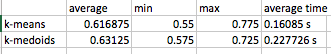
\includegraphics[scale=1.0]{datas.png}
\newline{}
While the k-means algorithm attains a higher maximum performance across 10 iterations, the k-medoids algorithm does better on average and has a higher minimum performance. In terms of runtime, the k-means algorithm beat out the k-medoids algorithm, with runtimes of 0.16 and 0.22 seconds respectively. 
}

\item Problem 3b

\solution{
The following plot shows the clustering score versus the number of principal components for both algorithms: \newline{}
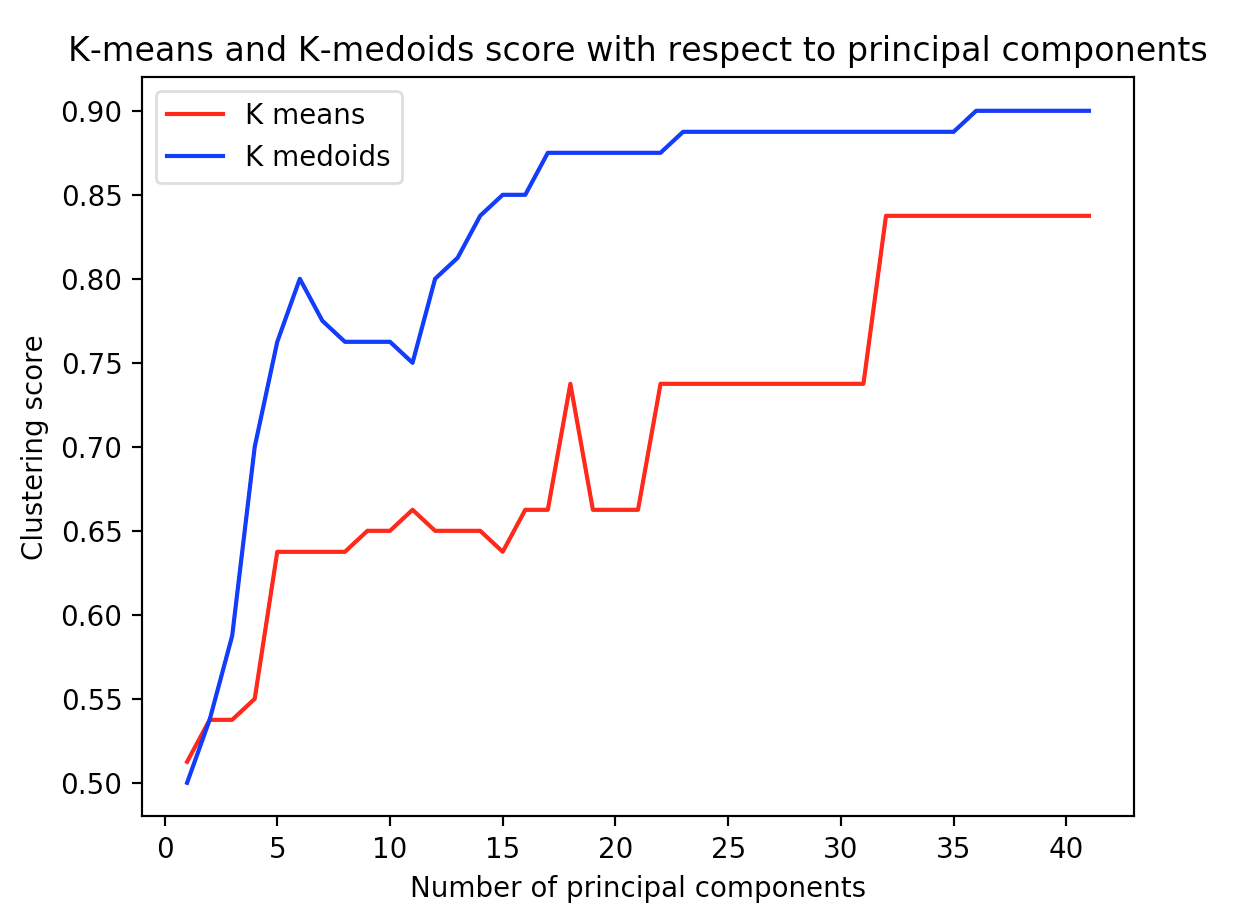
\includegraphics[scale=0.7]{kmeans-meds-pca-l-range.png} \newline{}
In general, both algorithms' performance increases as we increase the number of principal components; however, the performance plateaus as $l = 41$ is approached. This makes sense - with a small number of principal components, the data belonging to the two classes will not separate very well since only a few features was not enough for the algorithm to distinguish between the two classes well. However, as we increase the number of principal components, the dataset we run the clustering algorithm on has more and more features, which allows the algorithm to distinguish between the two classes better. \newline{}
The k-medoid algorithm attains higher performance than the k-means algorithm for all values of $l$ besides $l = 1, 2$ (approximately). This leads us to the supposition that using medoids, which are actual points in the dataset (the point whose distance to all other points is the least), to define the "centers" for our clusters yields better performance (on this particular dataset) than computing the "average" point (centroid) which is usually not in the dataset. 
}

\item Problem 3c

\solution{
For this problem, we had to find a pair that corresponds to the highest clustering score amongst all pairs, and another pair that corresponds to the lowest clustering score amongst all pairs. To do this, I iterated through all possible pairs of (0,18) inclusive (with a nested for loop), ran the k-medoids clustering algorithm, and called the score() function in the ClusterSet to compute the score. I then kept track of the highest and lowest currently found scores, and the associated pairs. 
\newline{}

Pair of labels that clustering can discriminate very well (corresponding to the highest score) was (9, 16) with score 0.9875: \newline{}
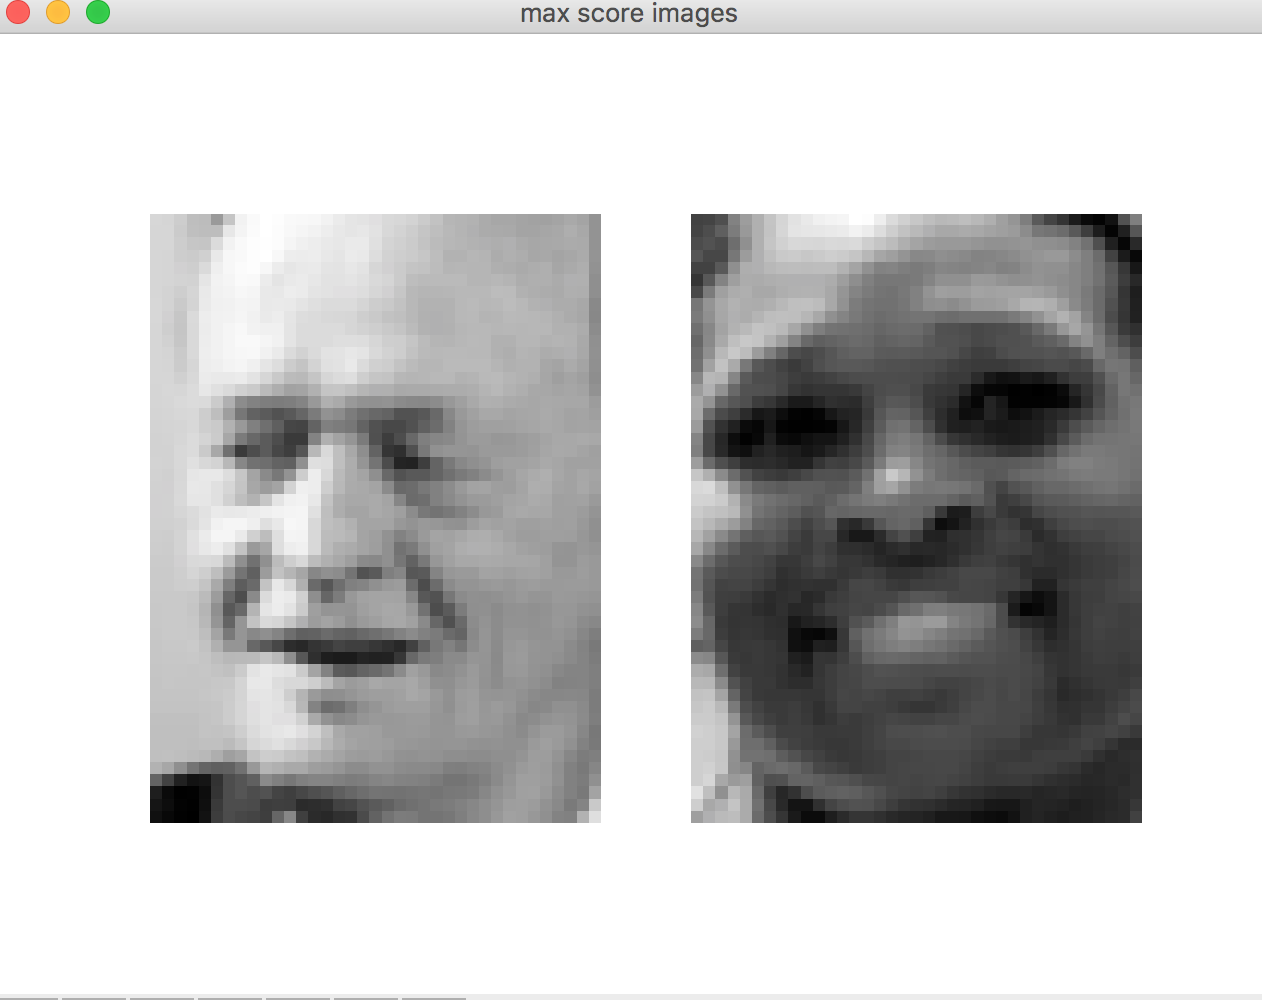
\includegraphics[scale = 0.6]{max-score-image.png} \newline{}

Pair of labels that clustering cannot discriminate well (corresponding to the lowest score) was (4, 5) with score 0.5125: \newline{}
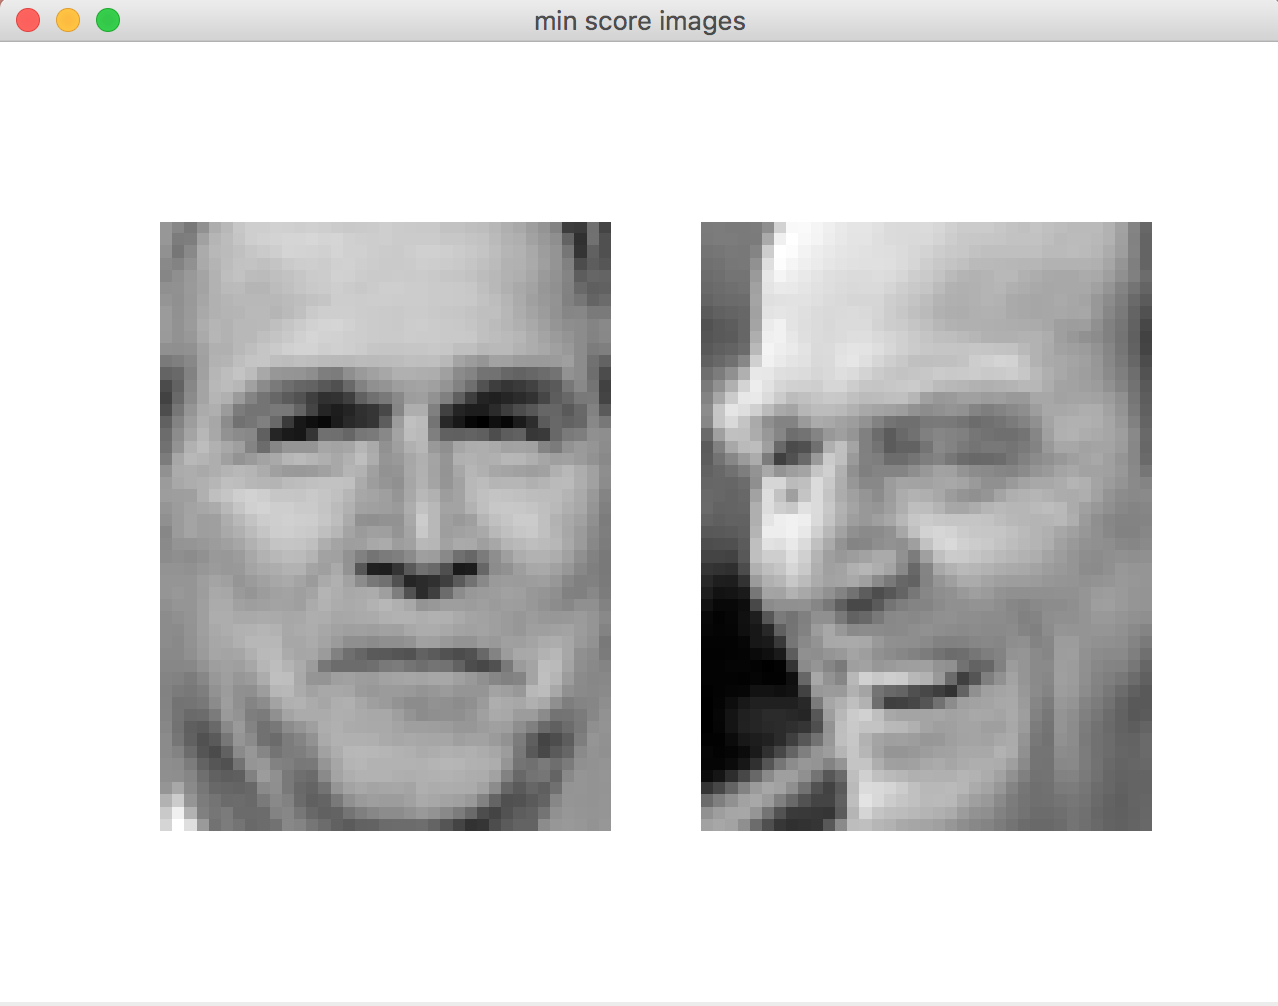
\includegraphics[scale = 0.6]{min-score-image.png}

\newline{}

We see that two faces that look very different (in terms of both color and facial feature structure) corresponded to the highest clustering score. Clustering (with k-medoids) was able to distinguish between these two faces very well - in $D$ dimensional space, their corresponding features would be very well separated with respect to each other. On the other hand, for the minimum score pair of faces, the two faces look very similar, both in terms of facial structure, facial expression, color, and features (eyes, nose, mouth). The two pairs actually seem like the same person, but one picture was taken at a different angle. Clustering was not able to distinguish between these two classes well at all, having only a score of 0.5. In $D$ dimensional space, their corresponding features would not be well separated at all. 


}
\end{document}
